\section{Kollaboration}\label{section:konzeption:kollaboration}

\usetikzlibrary{arrows.meta}

% \begin{note}
%     \textbf{Notizen:}
%     \begin{itemize}
%         \item Erwähnung von \autoref{requirement:Kollaboration}
%         \item Beschreibung der grundlegenden Konzepte
%         \item Klassendiagramm kollaborative Datentypen
%         \item Klassendiagramm Collaboration Service \& dazugehörige Klassen
%         \item Beschreibung der verschiedenen Interaktionen zwischen Producer und Consumer
%               \begin{itemize}
%                   \item Beginn der Synchronisation
%                   \item Synchronisation des geteilten JSON-Objekts
%                   \item Austausch von Zustandsinformationen
%                   \item high-level Sequenzdiagramme + low-level Beschreibung
%               \end{itemize}
%         \item Beschreibung der Einbindung in die betrachtete Experimentkonfiguration
%         \item Nutzung von JSON-Schema für Beschreibung des geteilten JSON-Objekts
%     \end{itemize}
% \end{note}

Nach \autoref{requirement:Kollaboration} soll die IDE die Echtzeit-Kollaboration mit anderen Laborgeräten innerhalb eines Experiments unterstützen. Dafür soll laut Unteranforderung (a) ein entsprechender CrossLab-Service entwickelt werden. Dieser soll nach Unteranforderung (b) für die Ermöglichung der Echtzeit-Kollaboration von der IDE verwendet werden.

Es gibt viele verschiedene Methoden zur Synchronisierung von Daten zwischen mehreren Teilnehmern. Beispiele derartiger Methoden sind \emph{\ac{OT}} \cite{sun_operational_1998}, \emph{Differential Synchronization} \cite{fraser_differential_2009} und \emph{\acp{CRDT}} \cite{shapiro_conflict-free_2011}. Aufgrund der Tatsache, dass jede dieser Methoden eigene Vor- und Nachteile besitzt, sollte die entwickelte Lösung möglichst unabhängig von dem zugrunde liegenden Synchronisationsalgorithmus sein, damit für den jeweiligen Anwendungsfall der passende Algorithmus verwendet werden kann\todo{Feedback einholen}. Daher werden zunächst die grundlegenden Konzepte beschrieben, bevor der entwickelte CrossLab-Service vorgestellt wird.

\begin{figure}[tbp]
    \centering
    \resizebox{\textwidth}{!}{\begin{tikzpicture}
            \begin{interface}[text width=4cm]{CollaborationType}{0,0}
                \operation{+ toJSON()}
                \operation{+ onUpdate()}
            \end{interface}
            \begin{class}[text width=5cm]{CollaborationObject}{-6,2.25}
                \operation{+ setProperty()}
                \operation{+ getProperty()}
                \operation{+ deleteProperty()}
            \end{class}
            \begin{class}[text width=5cm]{CollaborationNull}{-6,-0.75}
            \end{class}
            \begin{class}[text width=5cm]{CollaborationArray}{-6,-2.25}
                \operation{+ push()}
                \operation{+ get()}
                \operation{+ delete()}
            \end{class}
            \begin{class}[text width=5cm]{CollaborationNumber}{6,2.25}
                \operation{+ set()}
            \end{class}
            \begin{class}[text width=5cm]{CollaborationString}{6,0}
                \operation{+ set()}
                \operation{+ insert()}
                \operation{+ delete()}
            \end{class}
            \begin{class}[text width=5cm]{CollaborationBoolean}{6,-3.35}
                \operation{+ set()}
            \end{class}
            \draw[umlcd style dashed line, -{Triangle[length=2.5mm,open]}] (CollaborationObject.east) -- ([yshift=5mm] CollaborationType.west);
            \draw[umlcd style dashed line, -{Triangle[length=2.5mm,open]}] (CollaborationNull.east) -- (CollaborationType.west);
            \draw[umlcd style dashed line, -{Triangle[length=2.5mm,open]}] (CollaborationArray.east) -- ([yshift=-5mm] CollaborationType.west);
            \draw[umlcd style dashed line, -{Triangle[length=2.5mm,open]}] (CollaborationNumber.west) -- ([yshift=5mm] CollaborationType.east);
            \draw[umlcd style dashed line, -{Triangle[length=2.5mm,open]}] (CollaborationString.west) -- (CollaborationType.east);
            \draw[umlcd style dashed line, -{Triangle[length=2.5mm,open]}] (CollaborationBoolean.west) -- ([yshift=-5mm] CollaborationType.east);
        \end{tikzpicture}}
    \caption{Klassendiagramm kollaborative Datentypen}
    \label{figure:klassendiagramm-kollaborative-datentypen}
\end{figure}

\begin{figure}[tbp]
    \centering
    \begin{tikzpicture}
        \begin{class}[text width=7cm]{CollaborationServiceProducer}{-4,0}
        \end{class}
        \begin{class}[text width=7cm]{CollaborationServiceConsumer}{4,0}
            \operation{+ getAwareness()}
            \operation{+ joinRoom()}
            \operation{+ executeTransaction()}
            \operation{+ valueToCollaborationType()}
            \operation{+ getProperty()}
            \operation{+ onUpdate()}
        \end{class}
        \begin{class}[text width=7cm]{Room}{0,-5}
            \attribute{+ awareness: Awareness}
            \operation{+ addParticipant()}
            \operation{+ removeParticipant()}
            \operation{+ valueToCollaborationType()}
            \operation{+ executeTransaction()}
            \operation{+ startSynchronization()}
            \operation{+ getProperty()}
            \operation{+ onUpdate()}
        \end{class}
        \begin{interface}[text width=7cm]{Awareness}{-4,-14}
            \operation{+ getLocalState()}
            \operation{+ setLocalState()}
            \operation{+ setLocalStateField()}
            \operation{+ getStates()}
            \operation{+ onChange()}
            \operation{+ onUpdate()}
        \end{interface}
        \begin{class}[text width=7cm]{AwarenessProvider}{-4,-11}
            \implement{Awareness}
            \operation{+ applyUpdate()}
            \operation{+ encodeStates()}
        \end{class}
        \begin{class}[text width=7cm]{CollaborationProvider}{4,-11}
            \operation{+ handleCollaborationMessage()}
            \operation{+ startSynchronization()}
            \operation{+ executeTransaction()}
            \operation{+ valueToColloraborationType()}
            \operation{+ getProperty()}
            \operation{+ onCollaborationMessage()}
            \operation{+ onUpdate()}
        \end{class}
        \draw[stroke] ([xshift=-10mm]CollaborationServiceProducer.south) -- ([xshift=-10mm] CollaborationServiceProducer.south |- , |- Room.west) -- (Room.west) node [above, xshift=-6mm] () {rooms} node [below, xshift=-4mm] () {0..*};
        \draw[stroke] ([xshift=10mm] CollaborationServiceConsumer.south) -- ([xshift=10mm] CollaborationServiceConsumer.south |- , |- Room.east) -- (Room.east) node [above, xshift=6mm] () {rooms} node [below, xshift=4mm] () {0..*};
        \draw[stroke] ([xshift=-5mm] Room.south) -- (-0.5,-10.5) -- (-4,-10.5) -- (AwarenessProvider.north) node [left, yshift=2mm] () {awarenessProvider} node [right, yshift=2mm] () {1};
        \draw[stroke] ([xshift=5mm] Room.south) -- (0.5,-10.5) -- (3.5,-10.5) -- ([xshift=-5mm] CollaborationProvider.north) node [left, yshift=2mm] () {1} node [right, yshift=2mm] () {collaborationProvider};
    \end{tikzpicture}
    \caption{Klassendiagramm Collaboration Service}
    \label{figure:klassendiagramm-collaboration-service}
\end{figure}

Im Folgenden wird für die Erklärung der Konzepte von mehreren an der Kollaboration teilnehmenden Clients und einem zentralen Synchronisationsserver ausgegangen. Die Clients besitzen die Möglichkeit, sogenannte \textit{Räume} zu erstellen bzw. ihnen beizutreten. Jeder Raum verwaltet ein geteiltes JSON-Objekt. Dieses nutzt Strings als Schlüssel mit entsprechenden kollaborativen Datentypen als Werten. Diese kollaborativen Datentypen sind in \autoref{figure:klassendiagramm-kollaborative-datentypen} dargestellt. \todo{ggf. Position anpassen}Dabei gibt es jeweils einen kollaborativen Datentypen für die JSON-kompatiblen Datentypen Object, Array, Number, String, Boolean und Null. Jeder kollaborative Datentyp bietet neben speziellen Funktionen zur Bearbeitung dessen auch eine Funktion zur Umwandlung in den zugrunde liegenden Datentyp sowie eine Funktion zur Registrierung von Event Handlern für \texttt{Update}-Events an. Änderungen an dem geteilten JSON-Objekt werden über den zentralen Server an die anderen Teilnehmer weitergeleitet. Zusätzlich können die Clients Zustandsinformationen an den Server melden, welcher diese ebenso an die anderen Clients weiterleitet. Die Zustandsinformationen der Clients sind ebenfalls JSON-Objekte, allerdings werden für diese die normalen JSON-Datentypen verwendet. Die Zustandsinformationen eines Clients können nur von diesem selbst verändert werden. Außerdem sollten die Clients ihre Zustandsinformationen regelmäßig aktualisieren. Clients können die Zustandsinformationen eines anderen Teilnehmers löschen, falls für eine gewisse Zeit keine Aktualisierung dieser vorgenommen wurde. Dadurch können z.B. Verbindungsabbrüche von Clients behandelt werden. Basierend auf diesen Konzepten wird nachfolgend der \textit{Collaboration Service} anhand bestimmter Szenarien vorgestellt. Im Nachfolgenden werden dabei auch die in \autoref{figure:klassendiagramm-collaboration-service} dargestellten Klassen und Funktionen erläutert.

\begin{figure}[tbp]
    \centering
    \resizebox{\textwidth}{!}{\begin{sequencediagram}
            \newthread{consumer1}{Consumer 1}
            \newthreadShift{producer}{Producer}{3cm}
            \newthreadShift{consumer2}{Consumer 2}{3cm}

            \begin{call}{consumer1}{trete Räumen bei}{consumer1}{}
            \end{call}
            \prelevel\prelevel
            \begin{call}{consumer2}{trete Räumen bei}{consumer2}{}
            \end{call}

            \begin{call}{consumer1}{Initialisierung}{producer}{}
                \begin{call}{producer}{registriere Consumer}{producer}{}
                \end{call}
            \end{call}
            \begin{call}{consumer1}{starte Synchronisation}{producer}{}
            \end{call}

            \begin{call}{consumer2}{Initialisierung}{producer}{}
                \begin{call}{producer}{registriere Consumer}{producer}{}
                \end{call}
            \end{call}
            \begin{call}{consumer2}{starte Synchronisation}{producer}{}
            \end{call}
        \end{sequencediagram}}
    \caption{Beispiel Initialisierung Synchronisation}
    \label{figure:initialisierung-synchronisation}
\end{figure}

Zunächst wird die Initialisierung der Synchronisation zwischen dem Collaboration Service Producer und dem Collaboration Service Consumer betrachtet. Dafür ist in \autoref{figure:initialisierung-synchronisation} ein möglicher Ablauf dargestellt. Zunächst tritt der Collaboration Service Consumer den Räumen bei, für welche er Daten bereitstellt bzw. welche in der Konfiguration der Verbindung mit dem jeweiligen Producer angegeben wurden. Dafür kann die Funktion \texttt{joinRoom()} des Collaboration Service Consumer verwendet werden. Der Beitritt in Räume kann auch nach dem Beginn der Synchronisation geschehen. Nachdem der Collaboration Service Consumer den Räumen beigetreten ist, sendet dieser eine Initialisierungsnachricht an den Collaboration Service Producer, welche u.a. einen einzigartigen Kennzeichner für den Collaboration Service Consumer beinhaltet. Dieser Kennzeichner kann entweder generiert werden oder über die Konfiguration der entsprechenden Laborgeräte während der Konfiguration des Experiments angegeben werden. Die Informationen der Initialisierungsnachricht werden von dem Collaboration Service Producer verwendet, um die Nutzer den entsprechenden Räumen zuzuordnen. Sobald der Collaboration Service Producer eine Antwort an den Collaboration Service Consumer gesendet hat, startet dieser die Synchronisation der einzelnen Räume über die Funktion \texttt{startSynchronization()}. Die Synchronisation erfolgt über die zugrunde liegende Synchronisationsmethode. Aufgrund dessen können Collaboration Service Consumer und Collaboration Service Producer nur verbunden werden, wenn sie die gleiche Synchronisationsmethode unterstützen.

\begin{figure}[tbp]
    \centering
    \resizebox{\textwidth}{!}{\begin{sequencediagram}
            \newthread{consumer1}{Consumer 1}
            \newthreadShift{producer}{Producer}{3cm}
            \newthreadShift{consumer2}{Consumer 2}{3cm}

            \begin{call}{consumer1}{ändere JSON-Objekt}{consumer1}{}
            \end{call}

            \begin{call}{consumer1}{sende Änderung}{producer}{}
            \end{call}

            \begin{call}{producer}{wende Änderung an}{producer}{}
            \end{call}

            \begin{call}{producer}{sende Änderung}{consumer2}{}
            \end{call}

            \begin{call}{consumer2}{wende Änderung an}{consumer2}{}
            \end{call}
        \end{sequencediagram}}

    \caption{Beispiel Synchronisation des geteilten JSON-Objekts}
    \label{figure:synchronisation-des-geteilten-json-objekts}
\end{figure}

Über die Funktion \texttt{getProperty()} des Collaboration Service Consumer kann der Zugriff auf die Eigenschaften des geteilten JSON-Objekts für einen spezifischen Raum erfolgen. Dabei wird zunächst die gleichnamige Funktion der Klasse \texttt{Room} aufgerufen, welche diesen Aufruf an den assoziierten \texttt{CollaborationProvider} weiterleitet. Der Rückgabewert der Funktion ist einer der zuvor erwähnten kollaborativen Datentypen. Es werden nur die Eigenschaften synchronisiert, die mindestens einmal über die Funktion \texttt{getProperty()} abgefragt wurden. Der erhaltene kollaborative Datentyp kann dann über dessen bereitgestellte Funktionen verändert werden, wobei kollaborative Objekte und Arrays nur kollaborative Datentypen als Eigenschaften bzw. Items unterstützen. Um einen unterstützten JSON-Datentypen in einen entsprechenden kollaborativen Datentypen umzuwandeln, kann die Funktion \texttt{valueToCollaborationType()} verwendet werden. Die Funktion \texttt{executeTransaction()} des Collaboration Service Consumers kann verwendet werden um mehrere Änderungen vorzunehmen, die dann in einem Update gesammelt werden. Updates und andere Nachrichten der zugrunde liegenden Synchronisationsmethode werden vom \texttt{CollaborationProvider} über ein entsprechendes \texttt{CollaborationMessage}-Event bekanntgegeben. Diese werden von dem dazugehörigen Raum behandelt. Die Nachrichten werden dabei an alle Teilnehmer des Raums gesendet. Eingehende Nachrichten der zugrunde liegenden Synchronisationsmethode können über die Funktion \texttt{handleCollaborationMessage()} des \texttt{CollaborationProvider} behandelt werden. Der weitere Verlauf der Synchronisation ist stark von der verwendeten Methode abhängig. Wenn alle Teilnehmer über Peer-to-Peer Verbindungen direkt miteinander verbunden sind, können die Updates eines Teilnehmers direkt an alle anderen gesendet werden. Dadurch ist keine Weiterleitung danach mehr nötig. Im Falle der Kommunikation über einen zentralen Server muss dieser die Änderung einzelner Teilnehmer an die anderen Teilnehmer weiterleiten. Wenn ein externes Update zur Änderung des geteilten JSON-Objekts führt, wird ein \texttt{Update}-Event vom \texttt{CollaborationProvider} ausgelöst. Event Handler für diese können über den Collaboration Service Consumer registriert werden.

\begin{figure}[tbp]
    \centering
    \resizebox{\textwidth}{!}{\begin{sequencediagram}
            \newthread{consumer1}{Consumer 1}
            \newthreadShift{producer}{Producer}{3cm}
            \newthreadShift{consumer2}{Consumer 2}{3cm}

            \begin{call}{consumer1}{ändere Zustand}{consumer1}{}
            \end{call}

            \begin{call}{consumer1}{sende Zustände}{producer}{}
            \end{call}

            \begin{call}{producer}{aktualisiere Zustände}{producer}{}
            \end{call}

            \begin{call}{producer}{sende Zustände}{consumer2}{}
            \end{call}

            \begin{call}{consumer2}{aktualisiere Zustände}{consumer2}{}
            \end{call}
        \end{sequencediagram}}

    \caption{Beispiel Austausch der Zustandsinformationen}
    \label{figure:austausch-der-zustandsinformationen}
\end{figure}

Die Zustandsinformationen für einen Raum können über die Funktion \texttt{getAwareness()} des Collaboration Service Consumers erhalten werden. Der lokale Zustand kann dann über die Funktionen \texttt{setLocalState()} und \texttt{setLocalStateField()} bearbeitet werden. Änderungen der Zustandsinformationen werden über \texttt{Update}- und \texttt{Change}-Events bekanntgegeben, wobei \texttt{Change}-Events nur ausgelöst werden, wenn sich die Zustandsinformationen tatsächlich verändert haben. Die Events werden vom Raum abgefangen und für die Weiterleitung der neuen Zustandsinformationen verwendet. Dafür ist in \autoref{figure:austausch-der-zustandsinformationen} ein entsprechendes Sequenzdiagramm dargestellt. Es werden immer alle vorhandenen Zustandsinformationen verschickt, wofür u.a. die Funktion \texttt{encodeStates()} des \texttt{AwarenessProvider} verwendet wird. Sobald die neuen Zustandsinformationen bei den entsprechenden Collaboration Service Producern ankommen, aktualisieren diese zunächst ihre bekannten Zustandsinformationen mithilfe der Funktion \texttt{applyUpdate()} des \texttt{AwarenessProvider}. Sollte dabei eine Änderung vorgenommen werden, wird eine entsprechende Nachricht an alle verbundenen Collaboration Service Consumer mit Ausnahme des ursprünglichen Senders des Updates verschickt. Die Behandlung von externen Updates ist identisch für Collaboration Service Consumer.

Für die Einbindung des Collaboration Service in die betrachtete Experimentkonfiguration gibt grundsätzlich zwei Möglichkeiten. Diese hängen von der verwendeten Synchronisationsmethode ab, wobei in beiden Fällen mindestens eine weitere Instanz der IDE hinzugefügt wird. Wenn ein zentraler Synchronisationsserver benötigt wird, muss dieser als ein entsprechendes Laborgerät in das Experiment eingebunden werden. Dabei bietet es einen Collaboration Service Producer an, während die IDEs einen entsprechenden Collaboration Service Consumer anbieten. Die zweite Variante geht von einer verteilten Synchronisationsmethode aus. Dabei bieten die IDEs sowohl einen Collaboration Service Producer als auch einen Collaboration Service Consumer an. Dadurch können diese direkt miteinander verbunden werden.

\begin{figure}[htbp]
    \centering
    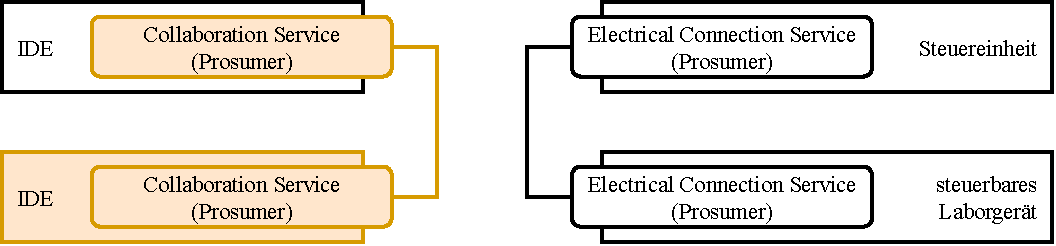
\includegraphics[width=\textwidth]{diagrams/experimentkonfigurationen/Experimentkonfiguration-01.drawio.pdf}
    \caption{Experimentkonfiguration}
    \label{figure:experimentkonfiguration:kollaboration}
\end{figure}